\chapter{Characterizing Adhesion in Multiple Myeloma Cells}
\label{Chap:Adhesion}\footnote{This chapter has been modified from draft of a manuscript. The manuscript includes as authors Theodorus de Groot, Jay Warrick, William Mattison, Cailin Holein, Shigeki Miyamoto and David Beebe}

\section{Introduction}The ability of a cell to mechanically interact with its environment is critically important to almost all aspects of cell biology and plays critical roles in many processes from development to immune response \cite{Halbleib2006,Springer1990,Springer1987}. These mechanical interactions between cells and their environment are mediated by adhesion molecules present on a cell's surface which enable the cell to physically attach to surrounding cells and structural molecules present in the environment \cite{Hay2013, Gumbiner1996}. Cell adhesion mediates a cascade of downstream effects which can result in significant changes in cell function and behavior \cite{Schlie-Wolter2013}. Many cell types require adhesion to other cells or structural molecules for survival and a lack of adhesion or lack of the appropriate extracellular matrix (ECM) components can result in a specific form of apoptosis known as anoikis \cite{Gilmore2005}. Anoikis prevents cells growing in contextually inappropriate locations and is important for maintaining the integrity of tissues in the body \cite{Gilmore2005}. In cancer, resistance to anoikis removes a tumor cell's dependence on adherence for survival, is considered a hallmark of cancer and is believed to be a requirement for cell survival in the bloodstream leading to metastasis \cite{Paoli20133481}. Multiple myeloma (MM) is a hematopoietic malignancy where the enhanced adhesion characteristics to ECM components and other cells in the bone marrow microenvironment mark increasing capacity for the cancer to interact with its microenvironment advancing tumor progression, immune evasion, and drug resistance \cite{Chauhan1996, Damiano2000, Gorgun2013, Jourdan1998b, Shain2001}. Characterizing adhesion in multiple myeloma can lead to an understanding of how tumor cells acquire resistance to specific treatments, changes that occur once cells are adhered, and potentially provide information about steps in metastasis.

There are several techniques used to characterize adhesion but they all have tradeoffs which limit their impact. Macroscale adhesion assays are well-suited for characterizing adhesion properties of populations of cells. A typical macroscale adhesion assay involves functionalizing the surface of a well-plate with an ECM protein or cell-bound molecule, or even cell population and allowing the seeded cells to settle to the bottom where they may adhere to the surface. After an incubation time, cells are washed with a micropipette, non-adherent cells are washed away while adherent cells remain at the surface of the well-plate. This approach results in the fractionation of cells into two populations based on their adherence characteristics. The adherent and non-adherent populations can be separated and interrogated following the assay with biochemical characterization methods.

Beyond this technique there are several microscale approaches to characterizing adhesion in populations of cells. Unlike their macroscale counterparts, microscale adhesion assays offer the potential to collect quantitative data about shear stresses required to dislodge cells or prevent their adhesion and can provide single-cell resolution. Microscale adhesion assays typically involve functionalizing a microchannel with a protein, molecule, or cell type of interest and observing the channel using microscopy. Detachment assays are setup like their macroscale counterparts, first allowing cells to settle onto the surface then by observing individual cell detachment from the surface with increasing flow rates. Microscale attachment assays flow cells into functionalized microchannels and modulating the flow rate from high to low, observing the flow at which individual cells adhere to the surface \cite{Yang2013, Lamorte2012}.

Macroscale adhesion assays are best suited for populations of cells with binary adhesion characteristics. Since these assays require pipetting which ideally operate at a single shear rate (though there are many factors that will affect shear) cells are separated into only two subpopulations, subtleties within a heterogeneous population will be largely unobservable. The largest benefit of macroscale adhesion assays is their ease of use and the ability to retain or collect cells from both adherent and non-adherent populations for further characterization. Microscale assays perform well characterizing single cells and can elucidate subtleties and transitions within complex populations. Unfortunately, the microchannel design requires flow through a channel. Under continuous flow, cells that are not adherent over the course of the assay will be washed away downstream into the waste and post-assay characterization of individual cells is challenging \cite{C2IB20036H, Andersson2003, ELPS200305627}. 

In spite of cell-based microscale devices being touted for their ability to minimize reagent use, due to their design, microchannel-based adhesion assays end up losing many cells to waste. The large amount of cell waste prevents these highly quantitative platforms from being utilized to analyze small-sized samples such as those isolated from patients. Warrick \textit{et al.} was capable of developing a quantitative microscale adhesion analysis by using using controllable oscillatory flow within a microchannel, preventing cells from being washed away. \cite{Warrick2013}. This platform enables adhesion assays with limited samples but does not address the need to further characterize cells once their adhesion characteristics have been determined. We present an adhesion assay that utilizes the oscillatory flow technique developed by Warrick \textit{et al.} and adds further functionality by implementing technique using photo-crosslinkable gel to "freeze" cells \textit{in situ} immediately following the adhesion assay, allowing a unique ability relate single-cell protein levels to adhesion strength. We also demonstrate the ability to simultaneously test two populations of cells within the same device for increased sensitivity and robustness to sample and device variability. We apply and validate this technique to cell lines and to cells isolated from multiple myeloma patients to better understand how adhesion plays a role in MM disease progression and drug resistance. 

\section{Methods}

\subsection{Device fabrication and preparation}
Adhesion devices were fabricated according to the protocol used by Warrick \textit{et al.} \cite{Warrick2013} using polydimethylsiloxane for the channel layer and device membrane and slide glass for the floor of the device. Device assembly was achieved using two-sided tape that was pattered via tomography or 'razor-printing' using a plotter cutter \cite{Martinez2008a, Kim2009,Bartholomeusz2005}.

Devices were functionalized with three different surface treatments with molecules multiple myeloma cells have been reported adhering to in the bone marrow microenvironment. These surface treatments are VCAM, ICAM, and hyaluronic acid (HA). The devices were treated as follows: Device components were oxygen plasma treated at 50W for 30 seconds. Devices were then assembled on the benchtop then exposed to germicidal UV light for 20 minutes. In sterile conditions, devices were filled with 100 \textmu g/mL either VCAM, ICAM, or HA in 1X PBS. A control condition was filled with 1X PBS. Filled devices were placed in an incubator for 2 hours. Following incubation, devices were flushed with 1X PBS for at least three volume replacements then returned to the incubator for at least 1 hour before use.

In experiments using patient cells, CD138+ cells were isolated from patient bone marrow aspirates as described previously \cite{Pak2015}. Cell line experiments used the MM lines RPMI8226 and MM.1R. Prior to the adhesion assay being run RPMI8226 cells were stained with Hoechst and MM.1R cells were stained with cell tracker red so that they could be later identified and registered for surface marker characterization. 

Crosslinkable media was prepared using the PEG-diacrylate and lithium phenyl-2,4,6-trimethylbenzoylphosphinate photo-crosslinkable protocol as described by Fairbanks \textit{et al. } \cite{Fairbanks2009}. Cells were added to the media at 200 cells/\textmu L.

Devices were prepared for operation by first thoroughly washing the channels out with crosslinking media. 10 \textmu L of media was removed and replaced with 10 \textmu L of cell suspension. The device membrane is carefully placed on the outlet of the device and is tapped several times to ensure that a seal has been made and to distribute cells from the port into the channel. The loaded device is taken to the microscope where the assay is performed. 


\subsection{Platform operation}
The cell-loaded device was placed on the microscope and the tip of the piezo-actuator is placed in contact with the top of the membrane. The assay is performed by initiating programmed oscillation the piezo actuator and simultaneously beginning image acquisition. The oscillatory program sweeps in a sawtooth waveform from 1 Hz to 0.1 Hz over the course of 5 minutes. Shear stress and frequency are linearly related, increasing shear stress as the oscillation frequency increases. 

Following completion of the adhesion component of the assay, the field of view of the channel that was observed for the adhesion assay is exposed to UV light from the microscope's DAPI filter initiating crosslinking of the PEG in the channel fixing the cells in place allowing for further downstream single-cell quantification. By immobilizing the cells, adhesion results can be directly linked to results from immunostaining by registering the adhesion image data with the fluorescence microscopy data.

The device is disassembled by removing the PDMS lid from the glass bottom then the cells immobilized within the gel are fixed. The fixed cells can be further analyzed and characterized. 


\subsection{Adhesion analysis}

Images captured during the assay were processed using Je'Xperiment (JEX) an image processing suite that utilizes the ImageJ framework \cite{Warrick2016, Warrick2013}. Image sets were reduced in size (2 X 2 binning) to conserve memory and hard drive space. Images were processed to identify cells in each framed captured. Cells were saved as regions of interest (ROIs) with their x and y positions within the frame recorded and saved within text files. Text files containing the ROI data were processed in R via the University of Wisconsin HTCondor high throughput computer cluster. Cells or ROIs were tracked between frames using a custom developed particle tracking package for R. The particle tracking package enabled cells to be tracked throughout the course of the experiment from high to low flow rates and enabled the cell's velocity to be determined. Cells with a low enough velocity were considered adhered while those above the threshold velocity (3 pixels per 1/30 of an oscillation) were not adhered. The analyzed ROI files were collected form HTCondor where the analyzed data could be reviewed. 

Stained cells from the assay were imaged and registered to the final timepoint of the adhesion assay with a semi-automated coherent point drift registration algorithm based on \cite{Myronenko2010} and custom implemented as a new package for the R statistical software. 

\section{Results \& discussion}

The adhesion assay presented is based upon the one originally developed by Warrick \textit{et al.} though it brings several improvements. The first being increased control over the shear experienced by the cells in the channel. The driving signal for the piezo-actuator was changed from a sine-wave with variable shear through-out each period to a saw-tooth waveform for constant velocity between changes in direction. The signal generation was also simplified. Previously frequency of oscillation was controlled manually by a standard, but costly, laboratory frequency generator. Now, a 32-bit Arudino Due (Figure \ref{figure:AdFig1}A) which executes a programmed, repeatable, and robust cycle of high to low shear stresses at about 1/10$^{th}$ the cost. The Arduino was also critical for enabling cell immobilization after actuation. The scientific waveform generator could not be programmed beyond 500 s and could not hold the cells still after actuation to enable photo-crosslinking of the PEG gel. This programmable nature of the arduino enables use of consistent actuation parameters, simplifying use and data analysis. This assay also results in a large quantity of images being created for each channel run. The addition of frequency automation enables downsampling of the images acquired from approximately 8000 to 2000 images resulting in significant reduction of data set size without loss of adhesion information.

The physical device design (Figure \ref{figure:AdFig2}B) remains relatively unchanged from the previous version with the exception of the assembly method. The channel itself is now composed of a medical grade two-sided tape which has minimal height variation which is important to maintaining a constant shear between replicates. Additionally the two-sided tape reversibly bonds the PDMS "lid" of the device to the glass bottom. Being able to remove the lid of the device allows direct access to the culture after bonding, avoiding diffusion limitations through the gel and reducing staining protocol times from 1 week to 1 day. 


\begin{figure}[ht] %DONE
\centering
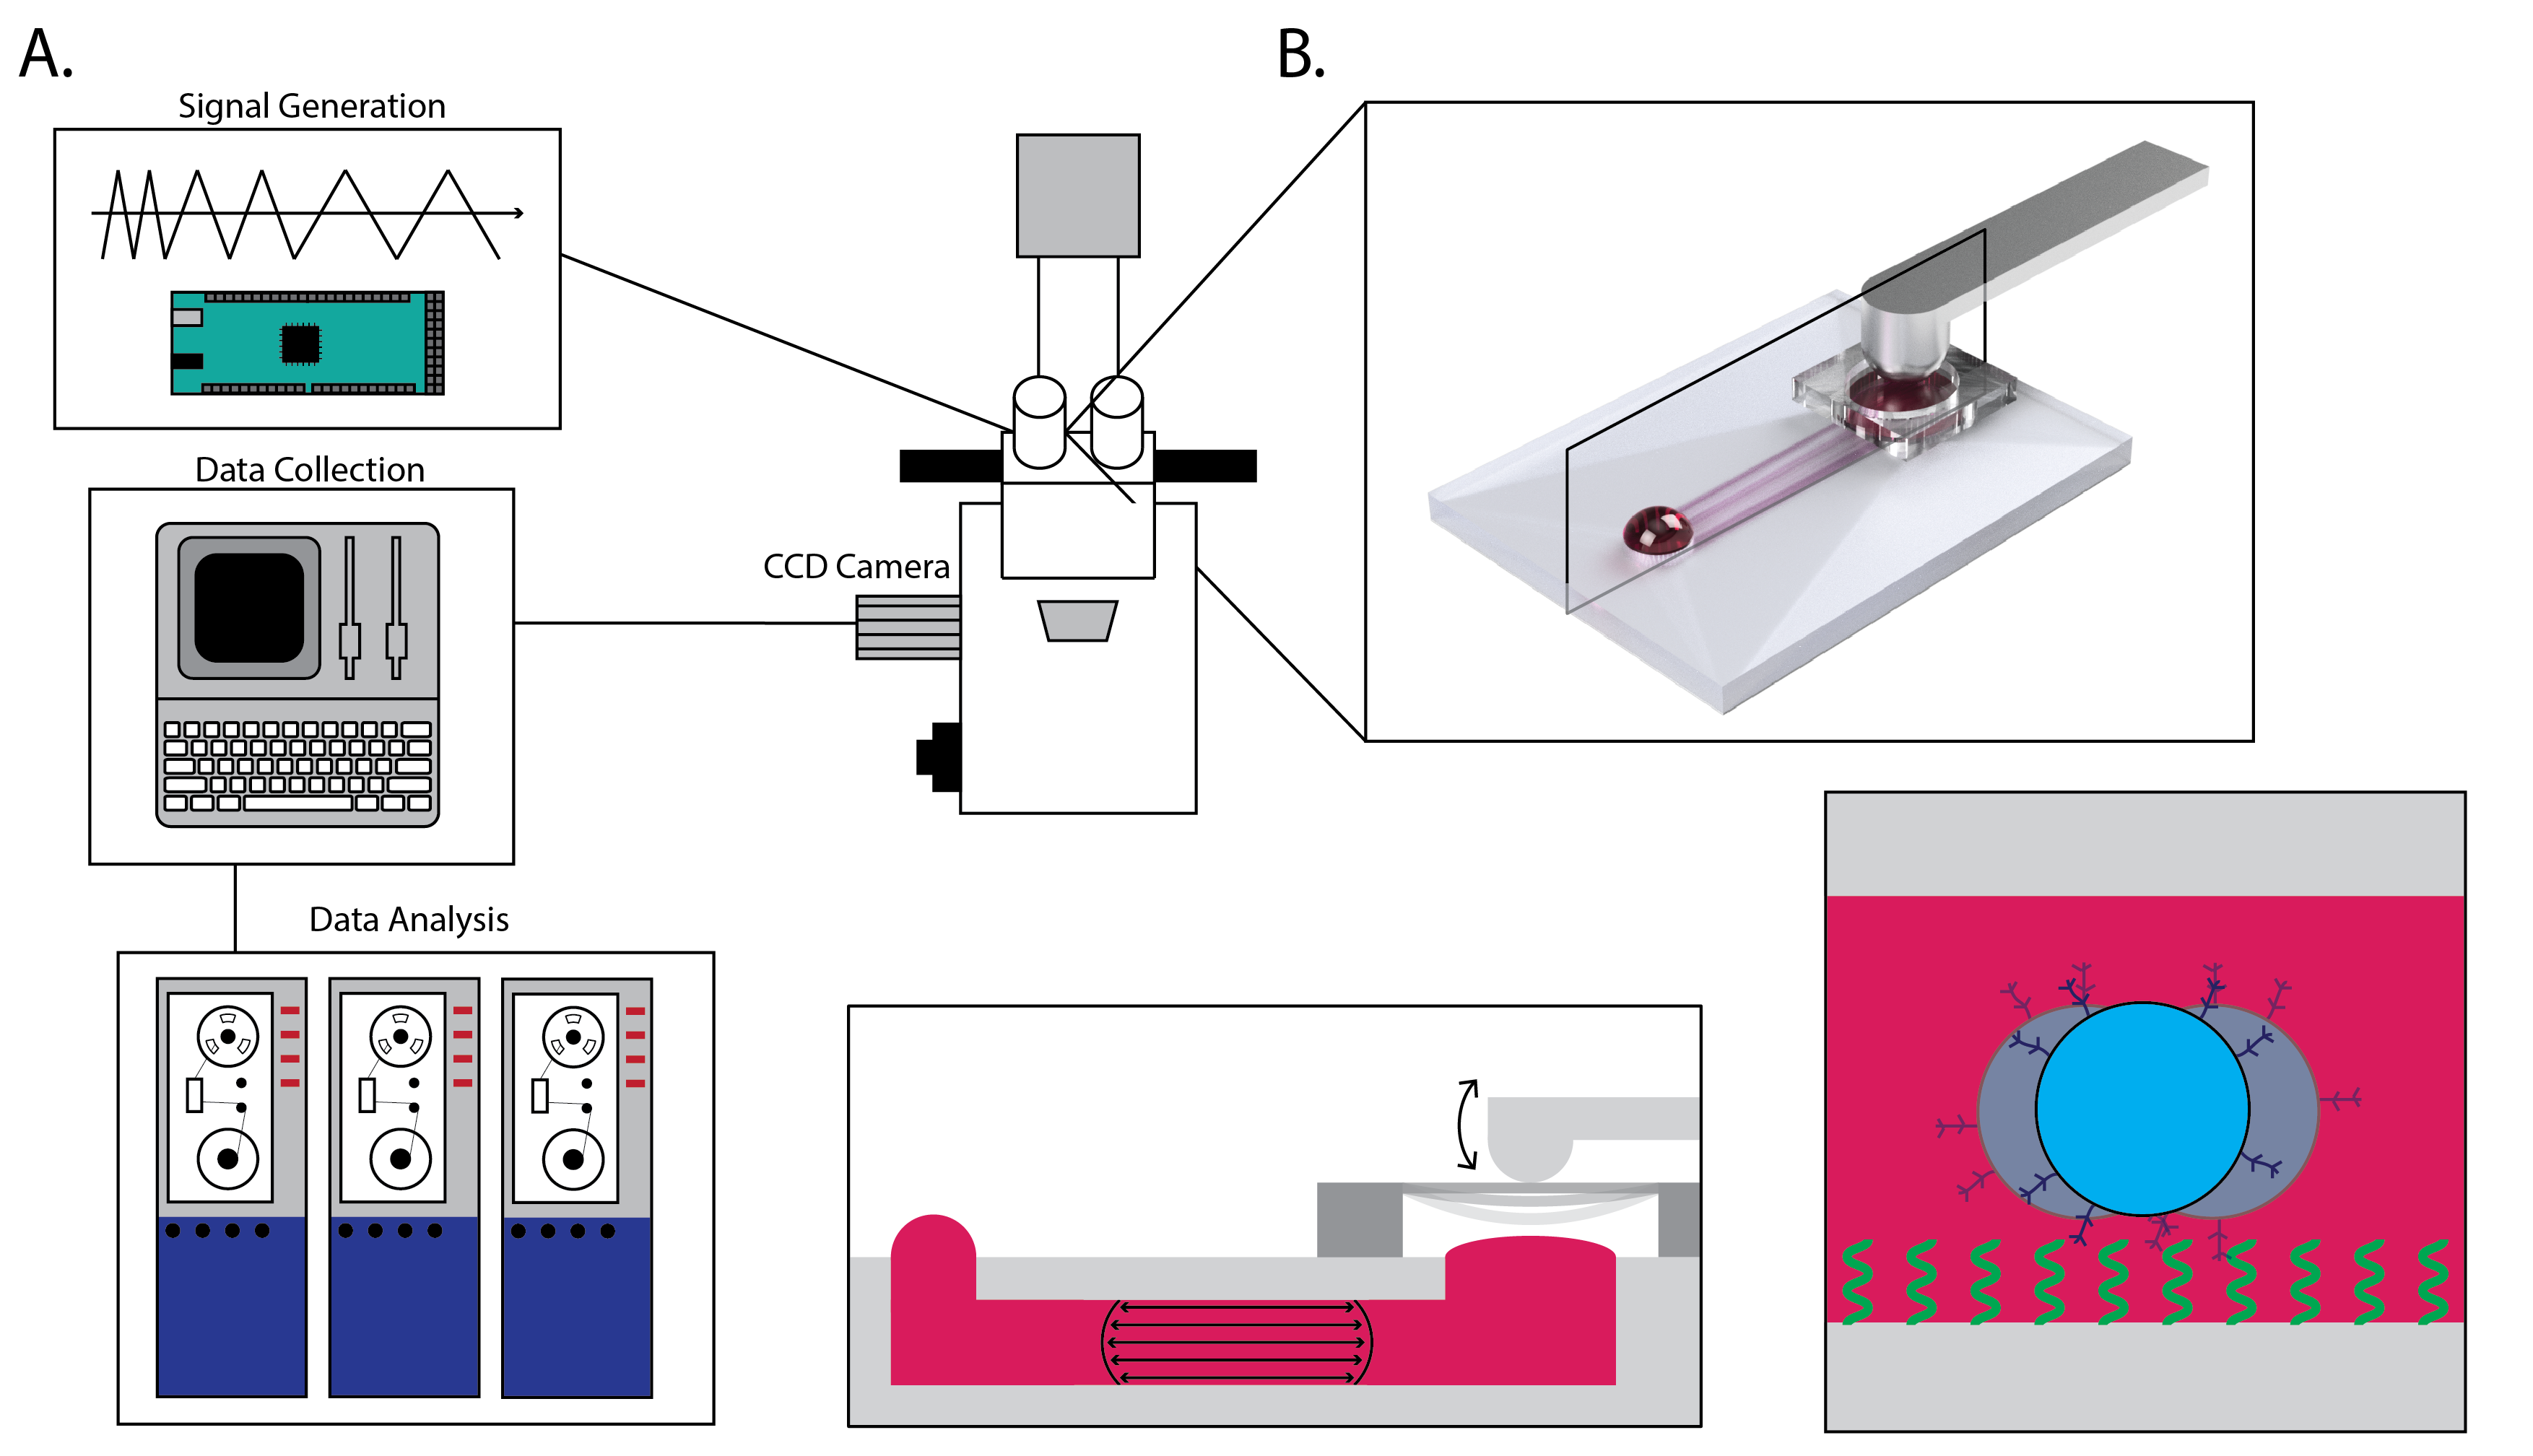
\includegraphics[width=5.75in]{/AdFig1.png}
\caption[\textbf{Adhesion assay schema}]{\textbf{Adhesion assay schema} A) Electronic components of adhesion assay. From top to bottom: Signal generator for piezo actuator, image collection from microscope-attached computer, data analysis performed by HTCondor. B) Adhesion device in increasing detail. From top to bottom: Complete adhesion channel with PDMS membrane and piezo actuator engaged, cross section of adhesion channel showing motion of actuator and fluid within the channel, representation of cell in channel oscillating on the surface of a functionalized channel.}
\label{figure:AdFig1}
\end{figure}

Prior to implementing the photo-crosslinking protocol we were able to analyze several MM patient samples with the adhesion assay with three relevant adhesion molecules found in the bone marrow microenvironemnt: VCAM, ICAM-1, and HA \cite{Hideshima2001, Damiano2000, Vincent2005, Reagan2012, Balakumaran2010, Ohwada2008, Vincent2005}. For example, VCAM is expressed on bone marrow stromal cells which mediates adhesion interaction with MM cells have shown to contribute to drug resistance \cite{Simmons1992}. We determined an average frequency of adhesion for each patient on each of the surfaces used (Figure \ref{figure:AdFig2}). To mitigate effects resulting from sample age, the order in which surfaces were tested was performed at random. The \emph{presentation} order of the data in Figure \ref{figure:AdFig2} is according to sample behavior with the first three samples having markedly higher mean adhesion frequency in the control condition as well as the VCAM condition and little adhesion in ICAM and HA conditions. The rightmost three samples shown no marked difference between conditions. These data, while interesting, alone are not enough to develop a well-formed mechanistic hypotheses and will require comparing to patient history and diagnosis to determine relevance. Furthermore, the following experiments to enable correlation of adhesion with cell staining endpoints illustrate that such advancements will likely be needed to provide sufficient control of experimental and biological variables for sensitive insight into complex and heterogeneous patient samples.

\begin{figure}[ht] %DONE
\centering
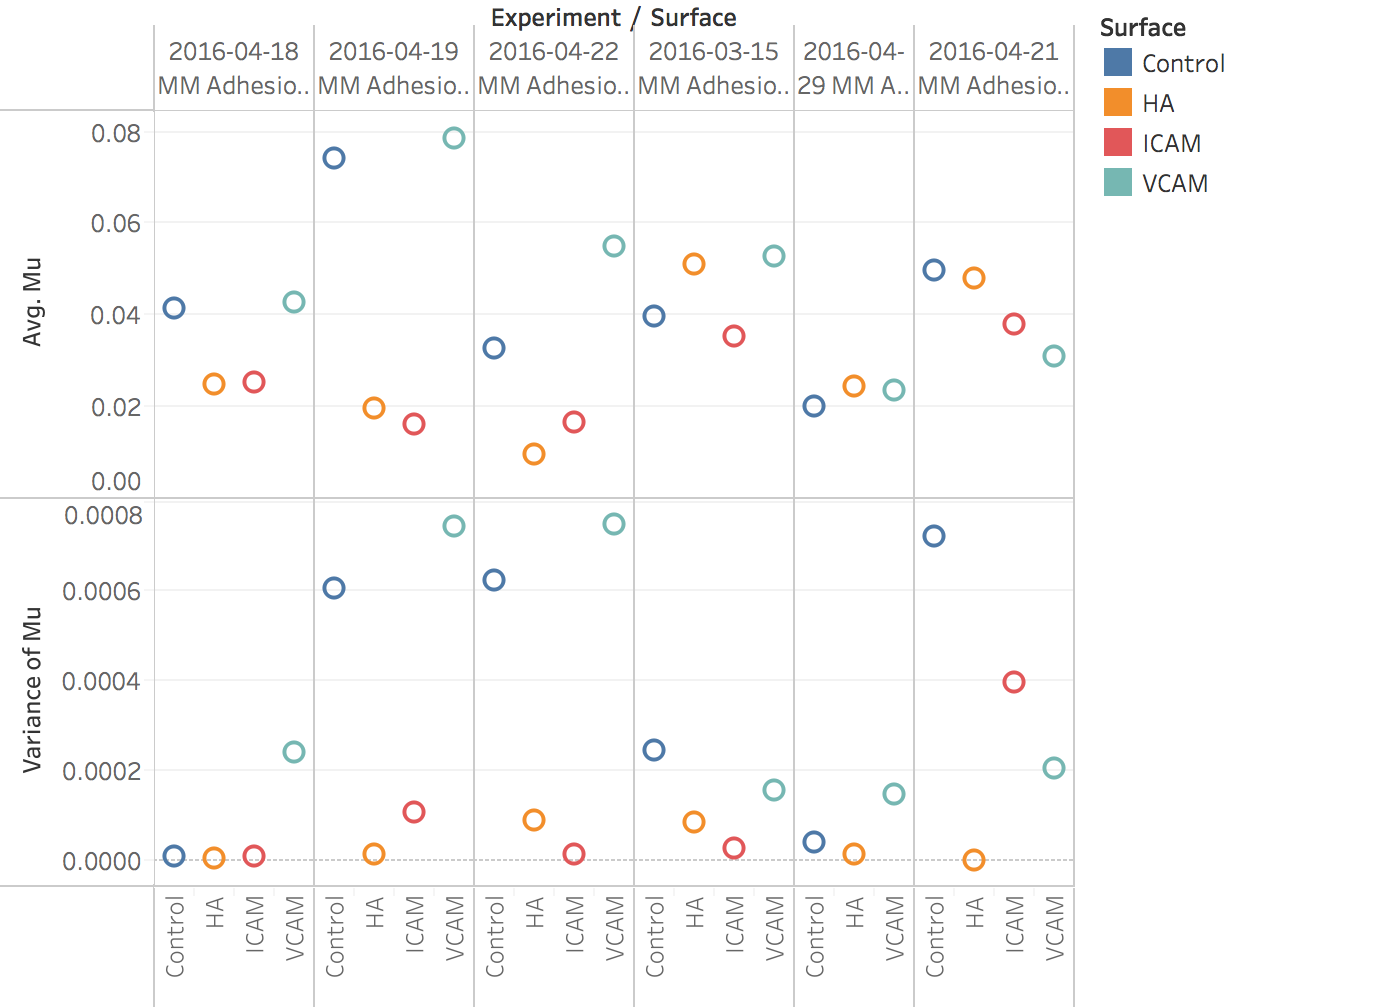
\includegraphics[width=5.75in]{/AdFig2.png}
\caption[\textbf{Aggregate patient adhesion data}]{\textbf{Aggregate patient adhesion data} Top: Frequency of oscillation at which average cell adheres to surface of channel bottom. Bottom: Variance of mean adhesion frequency for each condition and patient.}
\label{figure:AdFig2}
\end{figure}

To fully leverage the abilities of this adhesion platform, we developed software approaches to enable characterization of individual cells within each sample population. Looking at single cells within a channel, how they adhere, what their expression profile is, and the variablity between channels we can have a better understanding of the limitations of the assay and how the analysis can be performed to retrieve the most relevant results. We achieved this using the photo-crosslinking protocol to "freeze" cells in place and perform immunocytochemistry on them following completion of the adhesion assay. For these experiments we chose a focused system to analyze. We used only the control and ICAM surface conditions, compared adhesion and CD11 and CD227 surface staining between RPMI8226 (RPMI) and MM.1R cell lines. The two cell types are differentially labeled using live-cell tracer dyes Hoechst and CellTracker Red so that the cell type of each cell in the assay can be determined and used to enhance subsequent single-cell analysis.

Figure \ref{figure:AdFig3} A and B plot CD11a expression as a function of frequency of adhesion between channels. These data indicate a slight, though not dramatic dependence based on the channel the assay was performed in. This could be indicative of variability in the physical device\slash assay or other factors such changes in the cells after initial preparation of the stock cell suspension and sequential testing over the course of about 2 hours. Figure \ref{figure:AdFig3} C, which shows expression of both CD227 and CD11a across all replicates, appears distributed fairly similarly across the different channels. When the points are colored according the cell type, there are apparent differences in expression between the cell types. These data suggest that variability in staining expression is more dependent on cell type than the channel in which the staining was performed. In contrast, the observed adhesion strength was more dependent upon the channel than the cell type. However, we have not yet leveraged the ability to use the single-cell data to look for differences between populations within each channel individually in order to normalize channel-to-channel for variability.

Statistical analysis within each channel is performed using the non-parametric Wilcox-Mann-Whitney test for comparing two populations. We then aggregate the non-parametric results of each channel to see overall significance across channels using Lehman's procedure as described in MStat \cite{NormanR.Drinkwater, Drinkwater2011} and custom implemented in the R statistical software. Overall, the channels show highly consistent differences between the MM.1R and RPMI cells. MM.1R had consistently lower adhesion strength, CD11a expression, and CD227 expression. Although not statistically significant in all microchannels, the directionality of the observed difference was highly consistent and the aggregate p-value was highly-significant, even if corrected for multiple comparisons. It should also be noted, that MM.1R and RPMI cells are considered non-adherent cell lines; thus, they require very sensitive approaches and slow flow rates to interrogate adhesion interactions. For example, in previous work by Warrick \emph{et. al}, RPMI cells exhibited attachment adhesion strengths roughly 5 times lower than PC3-MM2 prostate cancer cells to endothelial cell monolayers. Thus, despite channel-to-channel variability in adhesion strength that was larger than differences between cell types within a channel, our approach enables consistent and highly sensitive comparison of multiple cell populations within a single channel.

\begin{figure}[ht] %DONE
\centering
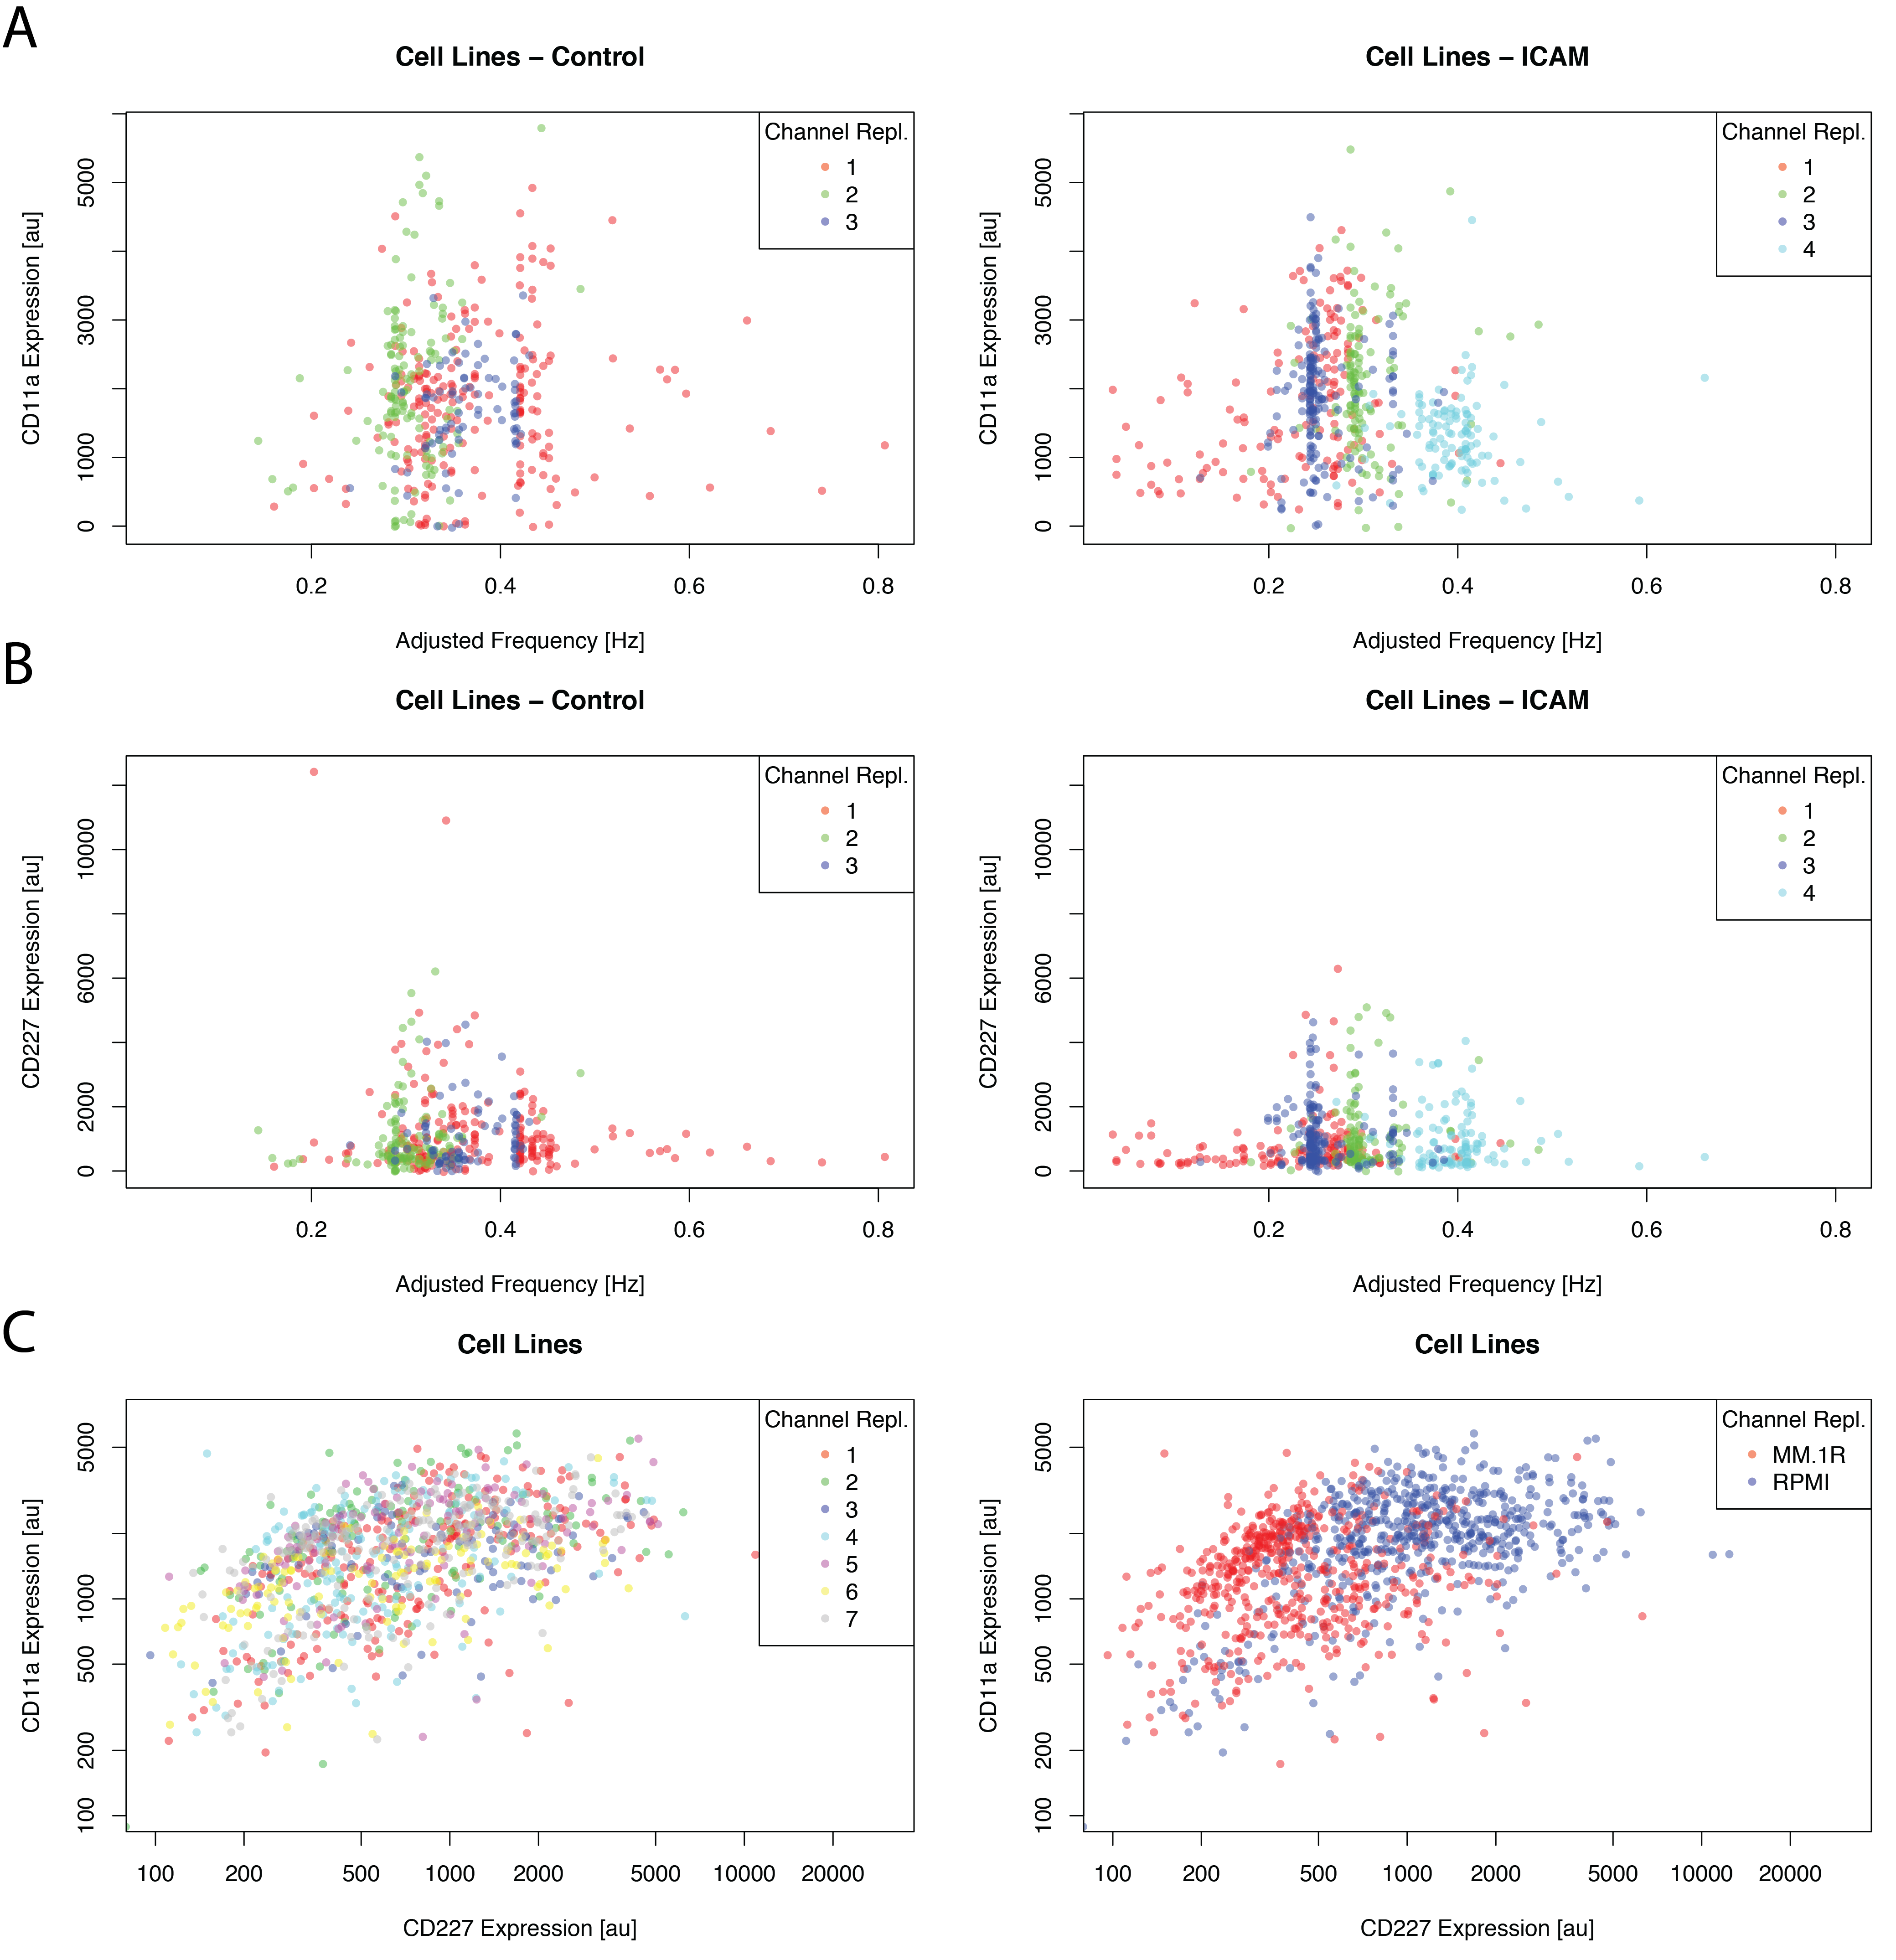
\includegraphics[width=5.5in]{/AdFig3.png}
\caption[\textbf{Surface marker expression and adhesion characteristics of MM cell lines, RPMI8226 and MM.1R}]{\textbf{Surface marker expression and adhesion characteristics of MM cell lines, RPMI8226 and MM.1R.} A) CD11a surface expression as a function of frequency of adhesion for control and ICAM surfaces. B) CD227 expression as a function of frequency of adhesion for control and ICAM surfaces. C) CD11a expression as a function CD227 for RPMI8226 and MM.1R cells across all replicates (left) and marked by cell line (right).}
\label{figure:AdFig3}
\end{figure}

We demonstrated the ability to perform single-cell analysis on a patient sample, again examining CD11a and CD227 expression and adhesion to control and ICAM surfaces using the same protocol as described for cell lines (Figure \ref{figure:AdFig4} A and B). However, in this case, we only have one population of cells to analyze. Instead, populations will need to be defined by expression. Given this type of analysis has not yet been performed on a patient sample, we first examine expression and adhesion variability across channels only.

Figure \ref{figure:AdFig4} illustrates that the variation in adhesion frequency is largely dependent on the replicate and channel used, much more markedly so than the cell lines. Thus, we suspect that patient MM tumor cells potentially degrade or change more rapidly with respect to adhesion than cell lines once isolated from patient marrow. Thus, the ability to perform analysis within each channel will be critical for observing trends in patient samples.

\begin{figure}[ht] %DONE
\centering
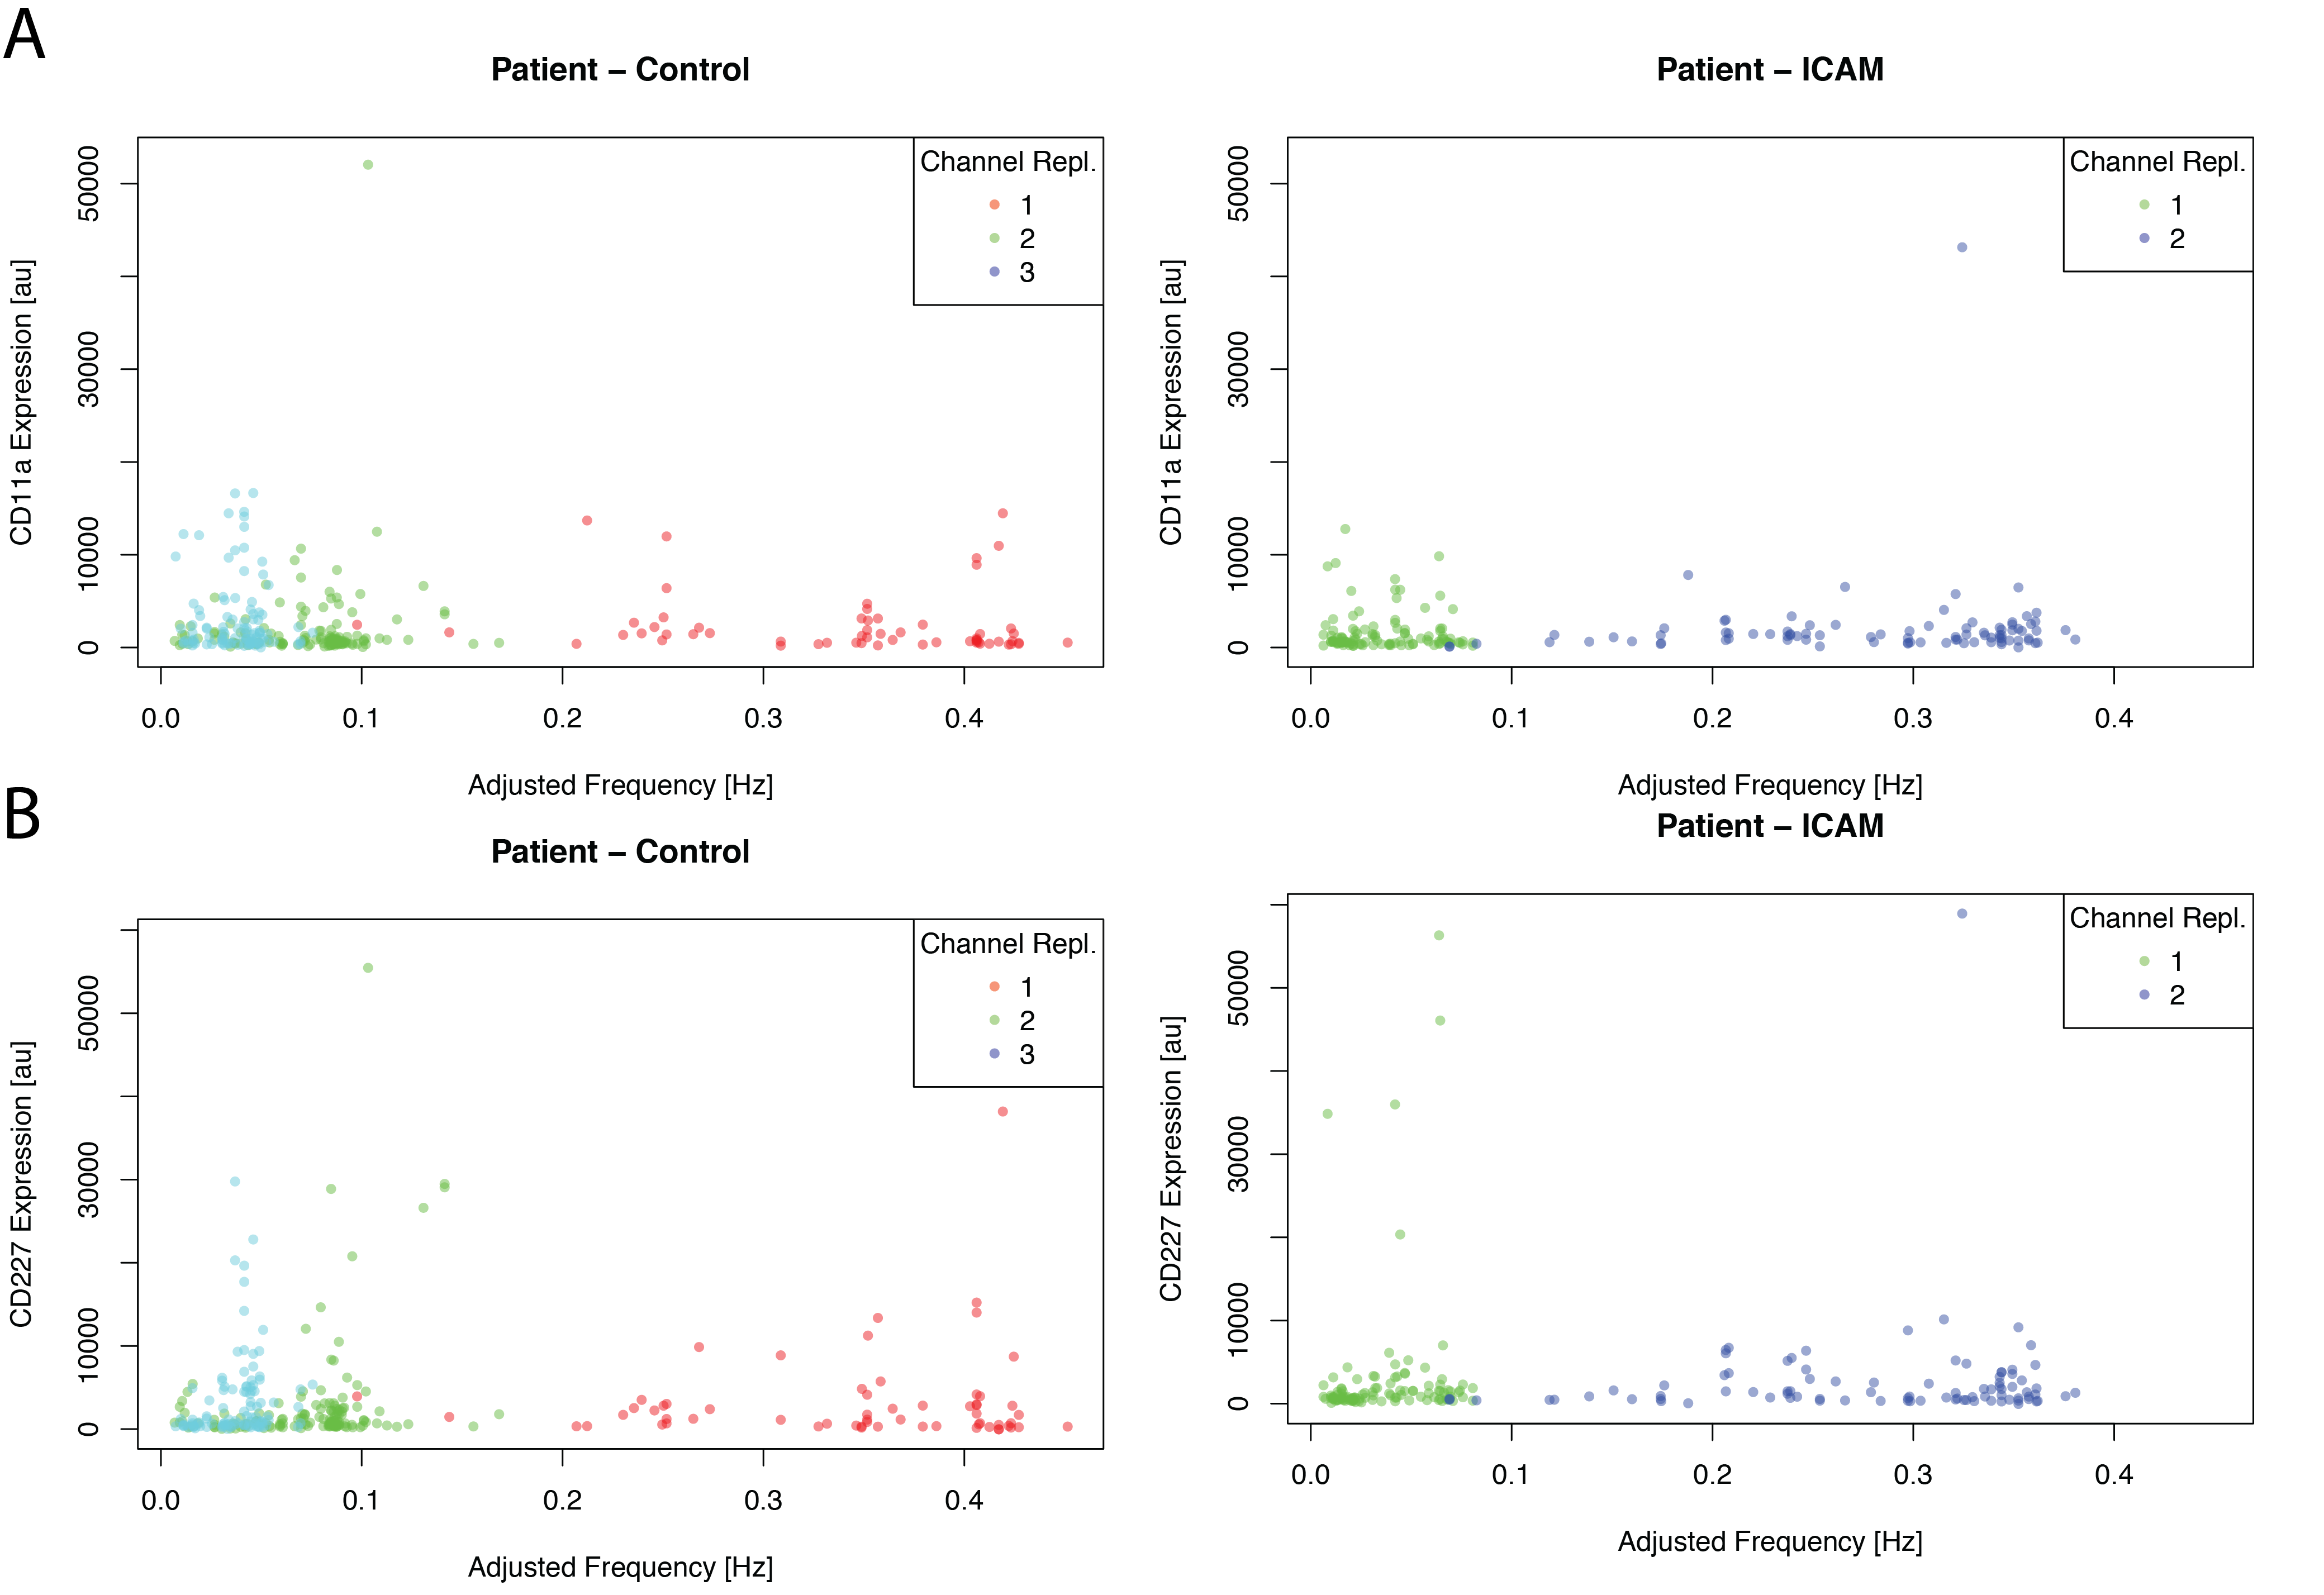
\includegraphics[width=5.5in]{/AdFig4.png}
\caption[\textbf{Surface marker expression and adhesion characteristics of a single MM patient sample}]{\textbf{Surface marker expression and adhesion characteristics of a single MM patient sample.} A) CD11a surface expression as a function of frequency of adhesion for control and ICAM surfaces. B) CD227 expression as a function of frequency of adhesion for control and ICAM surfaces. C) CD11a expression as a function CD227 for RPMI8226 and MM.1R cells across all replicates (left) and marked by cell line (right).}
\label{figure:AdFig4}
\end{figure}

To examine a potential relationship between CD227 and CD11a expression with MM tumor cell adhesion, we defined CD227-hi/lo and CD11a-hi/lo populations based upon whether they were above or below the median expression measured for that microchannel. Table \ref{tab:patientControl} and \ref{tab:patientICAM} summarize comparison of adhesion strength on the control and ICAM surface Using the same statistical procedure as used for comparing RPMI and MM.1R characteristics. We observed that patient cells higher in CD227 expression had higher adhesion strength to polystyrene where as they had lower adhesion to ICAM. Although the result is possibly counterintuitive, potentially the ICAM treatment is altering adsorption of an important ligand to the channel substrate. Likewise, it could be that CD227 does not play a large role during attachment but instead during detachment. At a higher level, the results show again, that single-cell analysis can find a statistically significant difference in adhesion amidst significant channel-to-channel variability that could arise for a variety of experimental and biological reasons. 


% MM1R vs. RPMI
% Overall p.value = 3.251435e-41 
% alpha.prime = 0 
% latex table generated in R 3.3.2 by xtable 1.8-2 package
% Wed Dec 14 12:38:05 2016
\begin{table}[ht]
\caption[Control-CD11a FADJ]{\textbf{Control-CD11a Fadj Overall p.value = 3.251435e-41\newline NOTE: FOR ALL TABLES IN THIS CHAPTER} Date is the data on which the data was acquired. Channel is the channel replicate on that date. U is the test statistic value of the Wilcox-Mann-Whitney test performed for that subset of data. z.score is the z-score of the test statistic value using a normal approximation for that data subset. p.value is the p-value is the z-score for that data subset. N is the number of cells in the data subset. p.symbol is the symbolic representation of the significance where * < 0.05, ** < 0.01, *** < 0.001. Difference is an indication whether the z-score is less than or greater than zero, indicating on whether the MM.1R cells were lower (-) or higher (+) than the RPMI cells for the given metric.}
\centering
\begin{tabular}{llrrlrll}
  \hline
Date & Channel & U & z.score & p.value & N & p.symbol & difference \\ 
  \hline
2016-08-10 & 0 & 496.00 & -2.18 & 0.250 &  77 &  & - \\ 
  2016-08-10 & 1 & 126.00 & -0.56 & 0.393 &  35 &  & - \\ 
  2016-08-10 & 2 & 119.00 & -2.00 & 0.428 &  40 &  & - \\ 
  2016-08-10 & 3 & 366.00 & -3.18 & 0.764 &  73 &  & - \\ 
  2016-08-16 & 0 & 3759.00 & -6.41 & 0.000 & 241 & *** & - \\ 
  2016-08-16 & 1 & 1454.00 & -4.75 & 0.002 & 147 & ** & - \\ 
  2016-08-16 & 3 & 514.00 & -4.65 & 0.068 & 100 &  & - \\ 
  2016-08-18 & 0 & 4488.00 & -8.64 & 0.000 & 418 & *** & - \\ 
  2016-08-18 & 2 & 1304.00 & -3.65 & 0.039 & 129 & * & - \\ 
   \hline
\end{tabular}
\end{table}

% MM1R vs. RPMI
% Overall p.value = 2.70024e-14 
% alpha.prime = 2.428058e-13 
% latex table generated in R 3.3.2 by xtable 1.8-2 package
% Wed Dec 14 12:38:05 2016
\begin{table}[ht]
\caption[Control-CD11a]{\textbf{Control-CD11a Overall p.value = 2.70024e-14}}
\centering
\begin{tabular}{llrrlrll}
  \hline
Date & Channel & U & z.score & p.value & N & p.symbol & difference \\ 
  \hline
2016-08-10 & 0 & 591.00 & -1.19 & 0.237 &  77 &  & - \\ 
  2016-08-10 & 1 & 187.00 & 1.49 & 0.139 &  35 &  & + \\ 
  2016-08-10 & 2 & 164.00 & -0.76 & 0.452 &  40 &  & - \\ 
  2016-08-10 & 3 & 638.00 & -0.14 & 0.890 &  73 &  & - \\ 
  2016-08-16 & 0 & 4092.00 & -5.79 & 0.000 & 241 & *** & - \\ 
  2016-08-16 & 1 & 1706.00 & -3.76 & 0.000 & 147 & *** & - \\ 
  2016-08-16 & 3 & 774.00 & -2.79 & 0.005 & 100 & ** & - \\ 
  2016-08-18 & 0 & 7942.00 & -4.96 & 0.000 & 418 & *** & - \\ 
  2016-08-18 & 2 & 2055.00 & -0.11 & 0.912 & 129 &  & - \\ 
   \hline
\end{tabular}
\end{table}

% MM1R vs. RPMI
% Overall p.value = 3.499617e-82 
% alpha.prime = 0 
% latex table generated in R 3.3.2 by xtable 1.8-2 package
% Wed Dec 14 12:38:05 2016
\begin{table}[ht]
\caption[Control-CD227.FADJ]{\textbf{Control-CD227.FADJ} Overall p.value = 3.499617e-82}
\centering
\begin{tabular}{llrrlrll}
  \hline
Date & Channel & U & z.score & p.value & N & p.symbol & difference \\ 
  \hline
2016-08-10 & 0 & 222.00 & -5.04 & 0.000 &  77 & *** & - \\ 
  2016-08-10 & 1 & 123.00 & -0.67 & 0.466 &  35 &  & - \\ 
  2016-08-10 & 2 & 98.00 & -2.58 & 0.130 &  40 &  & - \\ 
  2016-08-10 & 3 & 311.00 & -3.79 & 0.230 &  73 &  & - \\ 
  2016-08-16 & 0 & 2787.00 & -8.21 & 0.000 & 241 & *** & - \\ 
  2016-08-16 & 1 & 918.00 & -6.83 & 0.000 & 147 & *** & - \\ 
  2016-08-16 & 3 & 181.00 & -7.03 & 0.000 & 100 & *** & - \\ 
  2016-08-18 & 0 & 2540.00 & -10.72 & 0.000 & 418 & *** & - \\ 
  2016-08-18 & 2 & 451.00 & -7.67 & 0.000 & 129 & *** & - \\ 
   \hline
\end{tabular}
\end{table}

% MM1R vs. RPMI
% Overall p.value = 3.25774e-51 
% alpha.prime = 0 
% latex table generated in R 3.3.2 by xtable 1.8-2 package
% Wed Dec 14 12:38:05 2016
\begin{table}[ht]
\caption[Control-CD227]{\textbf{Control-CD227} Overall p.value = 3.25774e-51}
\centering
\begin{tabular}{llrrlrll}
  \hline
Date & Channel & U & z.score & p.value & N & p.symbol & difference \\ 
  \hline
2016-08-10 & 0 & 308.00 & -4.14 & 0.000 &  77 & *** & - \\ 
  2016-08-10 & 1 & 175.00 & 1.08 & 0.287 &  35 &  & + \\ 
  2016-08-10 & 2 & 116.00 & -2.08 & 0.036 &  40 & * & - \\ 
  2016-08-10 & 3 & 498.00 & -1.70 & 0.089 &  73 &  & - \\ 
  2016-08-16 & 0 & 3332.00 & -7.20 & 0.000 & 241 & *** & - \\ 
  2016-08-16 & 1 & 1113.00 & -6.07 & 0.000 & 147 & *** & - \\ 
  2016-08-16 & 3 & 311.00 & -6.10 & 0.000 & 100 & *** & - \\ 
  2016-08-18 & 0 & 5616.00 & -7.44 & 0.000 & 418 & *** & - \\ 
  2016-08-18 & 2 & 678.00 & -6.60 & 0.000 & 129 & *** & - \\ 
   \hline
\end{tabular}
\end{table}

% MM1R vs. RPMI
% Overall p.value = 2.014143e-18 
% alpha.prime = 0 
% latex table generated in R 3.3.2 by xtable 1.8-2 package
% Wed Dec 14 12:38:05 2016
\begin{table}[ht]
\caption[Control-FADJ]{\textbf{Control-FADJ} Overall p.value = 2.014143e-18}
\centering
\begin{tabular}{llrrlrll}
  \hline
Date & Channel & U & z.score & p.value & N & p.symbol & difference \\ 
  \hline
2016-08-10 & 0 & 280.50 & -4.43 & 0.000 &  77 & *** & - \\ 
  2016-08-10 & 1 & 66.00 & -2.61 & 0.104 &  35 &  & - \\ 
  2016-08-10 & 2 & 146.50 & -1.24 & 0.918 &  40 &  & - \\ 
  2016-08-10 & 3 & 327.50 & -3.61 & 0.350 &  73 &  & - \\ 
  2016-08-16 & 0 & 4531.00 & -4.98 & 0.016 & 241 & * & - \\ 
  2016-08-16 & 1 & 1565.00 & -4.32 & 0.008 & 147 & ** & - \\ 
  2016-08-16 & 3 & 456.00 & -5.06 & 0.015 & 100 & * & - \\ 
  2016-08-18 & 0 & 10457.50 & -2.28 & 0.000 & 418 & *** & - \\ 
  2016-08-18 & 2 & 2432.00 & 1.66 & 0.000 & 129 & *** & + \\ 
   \hline
\end{tabular}
\end{table}
% MM1R vs. RPMI
% Overall p.value = 1.449199e-39 
% alpha.prime = 0 
% latex table generated in R 3.3.2 by xtable 1.8-2 package
% Wed Dec 14 12:38:05 2016
\begin{table}[ht]
\caption[ICAM-CD11a.FADJ]{\textbf{ICAM-CD11a.FADJ} Overall p.value = 1.449199e-39}
\centering
\begin{tabular}{llrrlrll}
  \hline
Date & Channel & U & z.score & p.value & N & p.symbol & difference \\ 
  \hline
2016-08-10 & 0 & 1115.00 & -3.37 & 0.962 & 125 &  & - \\ 
  2016-08-10 & 2 & 88.00 & -4.82 & 0.288 &  63 &  & - \\ 
  2016-08-10 & 3 & 793.00 & 1.22 & 0.084 &  74 &  & + \\ 
  2016-08-16 & 0 & 2262.00 & -5.46 & 0.236 & 185 &  & - \\ 
  2016-08-16 & 1 & 947.00 & -5.51 & 0.000 & 131 & *** & - \\ 
  2016-08-16 & 2 & 824.00 & -5.52 & 0.000 & 127 & *** & - \\ 
  2016-08-16 & 3 & 2134.00 & -7.74 & 0.000 & 213 & *** & - \\ 
  2016-08-18 & 0 & 3782.00 & -5.24 & 0.771 & 478 &  & - \\ 
  2016-08-18 & 1 & 10806.00 & -1.92 & 0.035 & 548 & * & - \\ 
   \hline
\end{tabular}
\end{table}

% MM1R vs. RPMI
% Overall p.value = 3.56235e-05 
% alpha.prime = 0.0003205658 
% latex table generated in R 3.3.2 by xtable 1.8-2 package
% Wed Dec 14 12:38:05 2016
\begin{table}[ht]
\caption[ICAM-CD11a]{\textbf{ICAM-CD11a} Overall p.value = 3.56235e-05}
\centering
\begin{tabular}{llrrlrll}
  \hline
Date & Channel & U & z.score & p.value & N & p.symbol & difference \\ 
  \hline
2016-08-10 & 0 & 1790.00 & 0.14 & 0.890 & 125 &  & + \\ 
  2016-08-10 & 2 & 527.00 & 1.85 & 0.064 &  63 &  & + \\ 
  2016-08-10 & 3 & 832.00 & 1.64 & 0.101 &  74 &  & + \\ 
  2016-08-16 & 0 & 2877.00 & -3.76 & 0.000 & 185 & *** & - \\ 
  2016-08-16 & 1 & 1031.00 & -5.13 & 0.000 & 131 & *** & - \\ 
  2016-08-16 & 2 & 1006.00 & -4.63 & 0.000 & 127 & *** & - \\ 
  2016-08-16 & 3 & 2693.00 & -6.49 & 0.000 & 213 & *** & - \\ 
  2016-08-18 & 0 & 10272.00 & 2.91 & 0.004 & 478 & ** & + \\ 
  2016-08-18 & 1 & 16770.50 & 3.57 & 0.000 & 548 & *** & + \\ 
   \hline
\end{tabular}
\end{table}

% MM1R vs. RPMI
% Overall p.value = 2.121221e-76 
% alpha.prime = 0 
% latex table generated in R 3.3.2 by xtable 1.8-2 package
% Wed Dec 14 12:38:05 2016
\begin{table}[ht]
\caption[ICAM-CD227.FADJ]{\textbf{ICAM-CD227.FADJ} Overall p.value = 2.121221e-76}
\centering
\begin{tabular}{llrrlrll}
  \hline
Date & Channel & U & z.score & p.value & N & p.symbol & difference \\ 
  \hline
2016-08-10 & 0 & 773.00 & -5.14 & 0.012 & 125 & * & - \\ 
  2016-08-10 & 2 & 30.00 & -5.70 & 0.001 &  63 & *** & - \\ 
  2016-08-10 & 3 & 692.00 & 0.12 & 0.562 &  74 &  & + \\ 
  2016-08-16 & 0 & 1762.00 & -6.84 & 0.001 & 185 & ** & - \\ 
  2016-08-16 & 1 & 652.00 & -6.87 & 0.000 & 131 & *** & - \\ 
  2016-08-16 & 2 & 317.00 & -8.00 & 0.000 & 127 & *** & - \\ 
  2016-08-16 & 3 & 1406.00 & -9.37 & 0.000 & 213 & *** & - \\ 
  2016-08-18 & 0 & 1091.00 & -8.61 & 0.000 & 478 & *** & - \\ 
  2016-08-18 & 1 & 8718.00 & -3.85 & 0.654 & 548 &  & - \\ 
   \hline
\end{tabular}
\end{table}

% MM1R vs. RPMI
% Overall p.value = 4.520917e-37 
% alpha.prime = 0 
% latex table generated in R 3.3.2 by xtable 1.8-2 package
% Wed Dec 14 12:38:05 2016
\begin{table}[ht]
\caption[ICAM-CD227]{\textbf{ICAM-CD227} Overall p.value = 4.520917e-37}
\centering
\begin{tabular}{llrrlrll}
  \hline
Date & Channel & U & z.score & p.value & N & p.symbol & difference \\ 
  \hline
2016-08-10 & 0 & 1247.00 & -2.68 & 0.007 & 125 & ** & - \\ 
  2016-08-10 & 2 & 208.00 & -2.99 & 0.002 &  63 & ** & - \\ 
  2016-08-10 & 3 & 702.00 & 0.23 & 0.817 &  74 &  & + \\ 
  2016-08-16 & 0 & 2306.50 & -5.34 & 0.000 & 185 & *** & - \\ 
  2016-08-16 & 1 & 798.00 & -6.20 & 0.000 & 131 & *** & - \\ 
  2016-08-16 & 2 & 447.00 & -7.37 & 0.000 & 127 & *** & - \\ 
  2016-08-16 & 3 & 2029.00 & -7.98 & 0.000 & 213 & *** & - \\ 
  2016-08-18 & 0 & 3778.00 & -5.24 & 0.000 & 478 & *** & - \\ 
  2016-08-18 & 1 & 13457.50 & 0.52 & 0.606 & 548 &  & + \\ 
   \hline
\end{tabular}
\end{table}

% MM1R vs. RPMI
% Overall p.value = 1.803265e-19 
% alpha.prime = 0 
% latex table generated in R 3.3.2 by xtable 1.8-2 package
% Wed Dec 14 12:38:05 2016
\begin{table}[ht]
\caption[ICAM-FADJ]{\textbf{ICAM-FADJ} Overall p.value = 1.803265e-19}
\centering
\begin{tabular}{llrrlrll}
  \hline
Date & Channel & U & z.score & p.value & N & p.symbol & difference \\ 
  \hline
2016-08-10 & 0 & 1147.50 & -3.20 & 0.856 & 125 &  & - \\ 
  2016-08-10 & 2 & 167.00 & -3.61 & 0.062 &  63 &  & - \\ 
  2016-08-10 & 3 & 542.50 & -1.49 & 0.271 &  74 &  & - \\ 
  2016-08-16 & 0 & 1933.50 & -6.37 & 0.012 & 185 & * & - \\ 
  2016-08-16 & 1 & 1822.00 & -1.49 & 0.728 & 131 &  & - \\ 
  2016-08-16 & 2 & 1487.50 & -2.27 & 0.962 & 127 &  & - \\ 
  2016-08-16 & 3 & 3800.00 & -4.02 & 0.771 & 213 &  & - \\ 
  2016-08-18 & 0 & 4728.00 & -4.05 & 0.022 & 478 & * & - \\ 
  2016-08-18 & 1 & 12330.50 & -0.52 & 0.000 & 548 & *** & - \\ 
   \hline
\end{tabular}
\end{table}

% TRUE vs. FALSE
% Overall p.value = 2.417366e-17 
% alpha.prime = 0 
% latex table generated in R 3.3.2 by xtable 1.8-2 package
% Wed Dec 14 15:19:41 2016
\begin{table}[ht]
\caption[Patient-Control.FADJ]{\textbf{Patient-Control.FADJ} Overall p.value = 2.417366e-17 }
\centering
\begin{tabular}{llrrlrll}
  \hline
Date & Channel & U & z.score & p.value & N & p.symbol & difference \\ 
  \hline
2016-08-17 & 0 & 540.50 & 0.84 & 0.272 &  70 &  & - \\ 
  2016-08-17 & 1 & 2115.50 & 6.84 & 0.100 & 197 &  & - \\ 
  2016-08-17 & 2 & 914.50 & 5.75 & 0.007 & 132 & ** & - \\ 
   \hline
\end{tabular}
\label{tab:patientControl}
\end{table}

% TRUE vs. FALSE
% Overall p.value = 4.059469e-11 
% alpha.prime = 8.118928e-11 
% latex table generated in R 3.3.2 by xtable 1.8-2 package
% Wed Dec 14 15:19:41 2016
\begin{table}[ht]
\caption[Patient-ICAM.FADJ]{\textbf{Patient-ICAM.FADJ} Overall p.value = 4.059469e-11 }
\centering
\begin{tabular}{llrrlrll}
  \hline
Date & Channel & U & z.score & p.value & N & p.symbol & difference \\ 
  \hline
2016-08-17 & 1 & 1593.00 & -7.51 & 0.711 & 187 &  & - \\ 
  2016-08-17 & 3 & 1076.50 & -0.88 & 0.480 &  98 &  & - \\ 
   \hline
\end{tabular}
\label{tab:patientICAM}
\end{table}



\section{Conclusions \& future works}

This platform is highly versatile and is agnostic of cell type, meaning it isn't limited to hematopoietic cell types but can also be used to characterize adhesion in epithelial cells. The hardware and software controlling the assay and analysis can be reconfigured to run the assay in a detachment configuration which may be more appropriate for cells like multiple myeloma which have low observed adhesion strength in the attachment assay that was performed. In future work, it would be valuable to extend what we have learned here to enable further comparisons within each channel. For example, patterning of adhesion ligands within the channel (e.g., left-half and right-half) could allow direct comparison of cell-substrate affinity without the confounding effects of channel-to-channel variability. We also hope to differentially treat and pre-label fractions of patient samples for comparison within channels.